\chapter{Identificação de Elétrons}\label{cap:identificacao}

Um bom desempenho na reconstrução e identificação de elétrons é um ingrediente fundamental para o sucesso do programa científico do experimento ATLAS, uma vez que as principais assinaturas dos processos eletrofracos são os léptons \cite{alison2014road} e são utilizados para inúmeras análises, como, por exemplo, as medidas de precisão do modelo padrão, a descoberta do bóson de \emph{Higgs} e a busca por uma nova física além do Modelo Padrão \cite{aad2014electron}.


Os elétrons isolados produzidos em muitos do processos físicos de interesse estão sujeitos a uma grande quantidade de ruídos de fundo provenientes de:
\begin{itemize}
  \item Hádrons identificados equivocadamente;
  \item Fótons convertidos;
  \item Electrons não-isolados originados de decaimentos \emph{heavy-flavour}.
\end{itemize}

Por essa razão, é de primordial importância alcançar uma eficiente identificação de elétrons, sobre todo o detector e, ao mesmo tempo, manter uma grande rejeição de ruído de fundo.

\section{Reconstrução de Elétrons}\label{sec:rec_ele}

O algoritmo que efetua a reconstrução dos elétrons da região central ($|\eta| < 2,5$) do detector ATLAS identifica as energias depositadas no calorímetro EM e as associa aos traços do ID \cite{aad2014electron}, seguindo os três passos abaixo descritos:

\begin{enumerate}
  \item Reconstrução do \emph{Cluster}: o conjunto de células (do inglês \emph{cluster seed}) do EM provém das energias depositadas que contêm um total de energia transversa superior a 2,5 GeV, através de um algoritmo de janela móvel, com janela de tamanho 3x5 em unidades de 0,025 x 0,025 em $\eta$ x $\phi$;
  \item Combinar traço com conjunto de células: um traço e uma célula podem ser ditos combinados se a distância entre o ponto de impacto do traço e o baricentro da célula for $\Delta$$\eta$ < 0,05. E o tamanho de $\Delta$$\phi$ necessariamente precisa estar dentro de uma janela de 0.1;
  \item Candidato a elétron reconstruído: depois de combinar traço-célula, o tamanho do \emph{cluster} é otimizado para $\Delta$$\eta$ x $\Delta$$\phi$ = 3x7 (5x5) barril (tampa). O total da energia do candidato a elétron reconstruído é determinado pela soma de 4 fatores \cite{abat2008expected}:
      \begin{itemize}
        \item A energia estimada depositada na parte frontal do calorímetro EM;
        \item A energia depositada no \emph{cluster};
        \item A energia depositada fora do \emph{cluster} (também chamadas de perdas laterais);
        \item A energia depositada atrás do \emph{cluster} (perdas longitudinais).
      \end{itemize}
\end{enumerate}
	
A eficiência da reconstrução para os elétrons que passam pelo procedimento acima descrito é alta. Nesse estágio, da-se o nome de "\emph{reconstructed electrons }" aos candidatos que foram aprovados nos requisitos de \emph{cluster} e traço.

\subsection{\emph{Trigger} de Elétrons}
	
O sistema de \emph{Trigger} do ATLAS, como já mencionado na Seção~\ref{sec:sis_fil}, é constituído de três níveis, sendo que o L2 e EF juntos compõem a \ac{HLT}. No primeiro nível, selecionam-se somente os elétrons que ultrapassem um limiar de energia e, devido à dependência em $\eta$, esse limiar sofre variações \cite{alison2014road}.

O HLT utiliza as RoI preestabelecidas pelo L1; entretanto, um limiar mais refinado pode ser aplicado, bem como o uso de variáveis discriminantes, que serão apresentadas na Seção~\ref{sec:var_dis}.

Os pontos de operação do \emph{trigger} são definidos em três categorias:

\begin{itemize}
  \item \emph{Trigger} Primário: critérios rígidos são aplicados para coletar eventos de sinal em análise usando elétrons;
  \item \emph{Trigger} de Suporte: coletam amostras de elétrons não polarizados, utilizando basicamente E${_t}$ como critério;
  \item \emph{Trigger} para Monitoramento e Calibração: utilizados para coletar dados no intuito de garantir o correto funcionamento do \emph{trigger} e do detector \cite{aad2012performance}.
\end{itemize}


\section{Variáveis Discriminantes para Identificação de Elétrons}\label{sec:var_dis}

Tanto nas análises \emph{online} quanto \emph{offline}, critérios adicionais são aplicados no intuito de garantir uma melhor pureza dos elétrons reconstruídos. Estes critérios são informações retiradas dos calorímetros e do detector interno \cite{atlas2011expected} a partir de um conjunto de variáveis discriminantes, que podem ser dividas em:

\begin{itemize}
  \item Variáveis de Calorimetria;
  \item Variáveis de Traço;
  \item Variáveis de Traço-Calorimetria;
  \item Variáveis de Isolamento.
\end{itemize}

\subsection{Variáveis de Calorimetria}

As variáveis de calorimetria utilizam a fina segmentação lateral e longitudinal dos calorímetros do detector ATLAS:

\begin{itemize}
  \item Variável de vazamento hadrônico, R${_{had_1}}$:

  Definida como a razão entre as energias transversas da primeira camada do calorímetro hadrônico e do \emph{cluster}. Elétrons reais depositam mais energia no EM do que no HAD, apresentando assim valores pequenos de R${_{had_1}}$;

  \item Variável de largura em $\eta$ na segunda camada, ${W_{\eta 2}}$:

  É a medida da largura do chuveiro em $\eta$ ponderada pelo \ac{RMS} da distribuição em $\eta$ na segunda camada do EM. Esta variável contribui para suprimir ruído de fundo de jatos e conversões de fótons, que tendem a ter chuveiros maiores do que elétrons verdadeiros;

  \item Variável de largura do chuveiro, R${_\eta}$:

  É definida como a razão entre energia de uma janela 3x7 sobre uma janela 7x7, na segunda camada de amostragem.  Ruídos de fundo tendem a ter uma maior fração de energia fora do núcleo 3x7, resultando em baixos valores de R${_\eta}$.

  \item Variável de largura do chuveiro, R${_\phi}$:

  Semelhante à variável R${_\eta}$; entretanto, definida como a razão entre a energia em uma janela 3x3 sobre uma janela 3x7.

  \item Variável de largura do chuveiro na primeira camada do calorímetro, w${_{stot}}$:

  Mede a largura do chuveiro, que ajuda na identificação de elétrons porque apresenta maiores valores para ruído de fundo.

  \item Variável de razão de energia, E${_{ratio}}$.

  Também é utilizada para diminuir o ruído de fundo. É definida utilizando as células correspondentes às duas maiores energia nas camadas. Ruídos de fundo tendem a ter múltiplas incidências de partículas associadas, apresentando assim valores de E${_{ratio}}$ menores do que partículas de sinal.

  \item Fração de energia da terceira camada do EM, f${_3}$:

  Essa variável tende a ser menor para elétrons do que para ruído de fundo, uma vez que os elétrons não penetram tão profundamente no calorímetro.

  \item Fração de energia nas camadas do EM, f${_1}$:

  Essa variável é definida como a razão de energia depositada nas camadas sobre a energia total do EM.

\end{itemize}

A Figura~\ref{fig:3T01} mostra algumas das distribuições das variáveis acima apresentadas, bem como os vários tipos de ruídos de fundo.

\begin{figure}[h!]
	\centering
	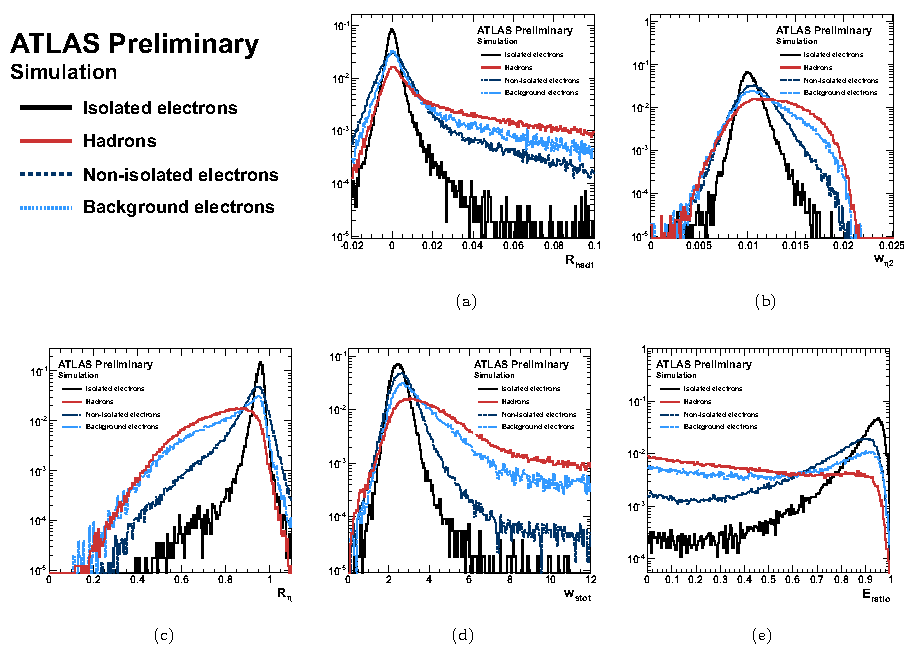
\includegraphics[width=14cm]{./textuais/identificacao/figuras/fig_1_variaveis_eletron.pdf}\\
	\caption{Variáveis de identificação de elétrons no calorímetro, formato do chuveiro, apresentados separadamente para sinal e os vários tipos de ruídos de fundo. As variáveis apresentadas são: (a) vazamento hadrônico R${_{had}}$, (b) de largura em eta no segundo W${_2}$ amostragem, (c) R${_\eta}$, (d) largura em $\eta$ nas w${_{s,tot}}$, pequeno, e (e) E${_{ratio}}$. Extraído de \cite{alison2014road}.}
	\label{fig:3T01}
\end{figure}

Essas variáveis são dependentes de $\eta$ e E${_t}$. Em $\eta$ devida à geometria dos calorímetros, que apresentam alguns pontos com menor resolução, como, por exemplo, a região, definida como \emph{crack}, que se encontra entre o barril e a tampa, 1,37 < |$\eta$| < 1,52, e que muitas vezes, é excluída de análises por conta da baixa resolução. Por outro lado, o poder de discriminação dessas variáveis melhora com o aumento de E${_t}$, uma vez que a largura do chuveiro tende a diminuir e o ruído de fundo tende a ter uma menor dependência de E${_t}$.

\subsection{Variáveis de Traço} \label{sec:variaveis_traço}

As variáveis de traço são provenientes do ID e podem ser utilizadas de forma a complementar as do calorímetro.
	
\begin{itemize}
  \item Número de \emph{hits} no detector Pixel (nPixHits) e Número combinado de \emph{hits} do Pixel e detectores de SCT (nSixHits):

      As camadas de detectores que são atravessadas por fótons antes de serem convertidos não têm traços associados a eles. Isso resulta em um menor número de \emph{hits} no detector de Pixels e SCT, do que os elétrons verdadeiros.

  \item Número de \emph{hits} na primeira camada do Detector de Pixels ou \emph{B-layer}:

  Essa variável apresenta uma sensibilidade a todas as conversões que ocorrem depois da primeira camada do Detector de Pixels, sendo bastante efetiva na redução de ruído de fundo.

  \item Parâmetro de impacto transverso, D${_0}$:

  Mede a distância mais próxima do traço do elétron até o vértice primário e possibilita a separação de conversões, dado que estes podem ter traços deslocados significativamente dos pontos de interação.

  \item Significância do parâmetro de impacto transverso, ${\sigma _{{d_0}}}$:

  Mede a relevância da distância mais próxima do traço do elétron até o vértice primário.

  \item \emph{Flag} de conversão, ou "bit conversão":

  É definido se o traço do elétron corresponde a um vértice de conversão. Reduz o número de elétrons reconstruídos de conversões, entretanto não é tão eficiente para elétrons verdadeiros.

  \item Fração de \emph{hits} de alto \emph{threshold} no TRT:

  Essa variável é uma das mais poderosas contra ruído de fundo provenientes de hádrons, em razão de mostrar a fração das detecção que passaram o limiar do detector TRT, indicando a presença de radiação de transição de fótons.

\end{itemize}

Na Figura~\ref{fig:3T02} são apresentadas algumas das variáveis de traço. Diferente das variáveis de calorimetria, as variáveis de traço são independentes de $\eta$ e E${_t}$, com exceção do TRT, e são pouco dependentes do \emph{pileup}.

\begin{figure}[h!]
	\centering
	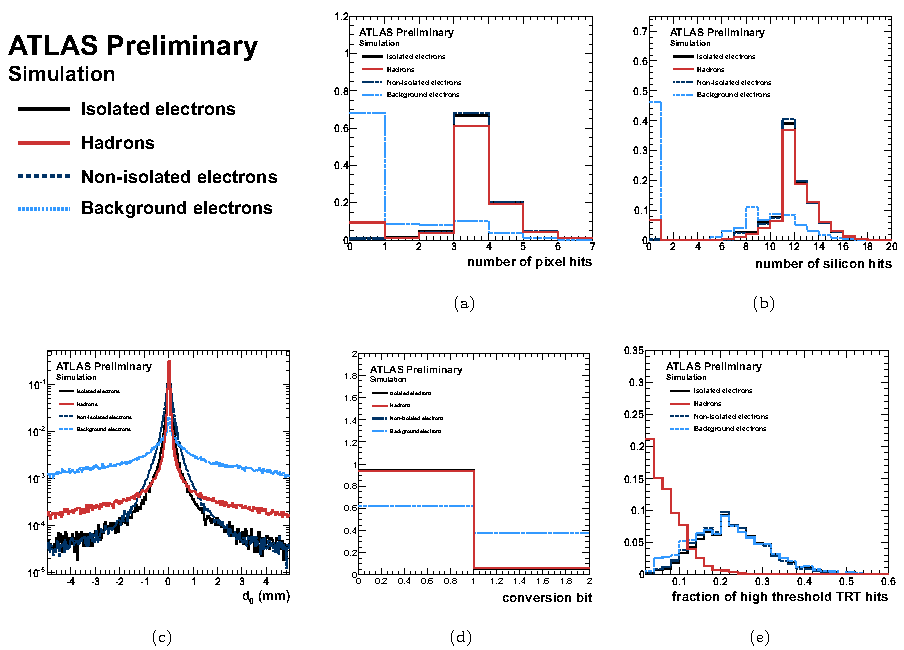
\includegraphics[width=14cm]{./textuais/identificacao/figuras/fig_2_variaveis_eletron.pdf}\\
	\caption{Variáveis de identificação elétron no ID, agrupados em sinal e vários tipos de ruídos de fundo. As variáveis apresentadas são: (a) número de \emph{hits} no detector Pixel, (b) número combinado de \emph{hits} do Pixel e detectores de SCT, (c) parâmetro de impacto transverso D${_0}$, (d) \emph{flag} de conversão, ou "bit conversão", e (e) fração \emph{hits} de alto \emph{threshold} no TRT. Extraído de \cite{alison2014road}.}
	\label{fig:3T02}
\end{figure}

\subsection{Variáveis de combinação Traço-Calorimetria}

Ao combinar as informações de traço e calorimetria, tem-se variáveis adicionais para discriminação de ruído de fundo. Essas são apresentadas na Figura~\ref{fig:3T03}.

\begin{figure}[h!]
	\centering
	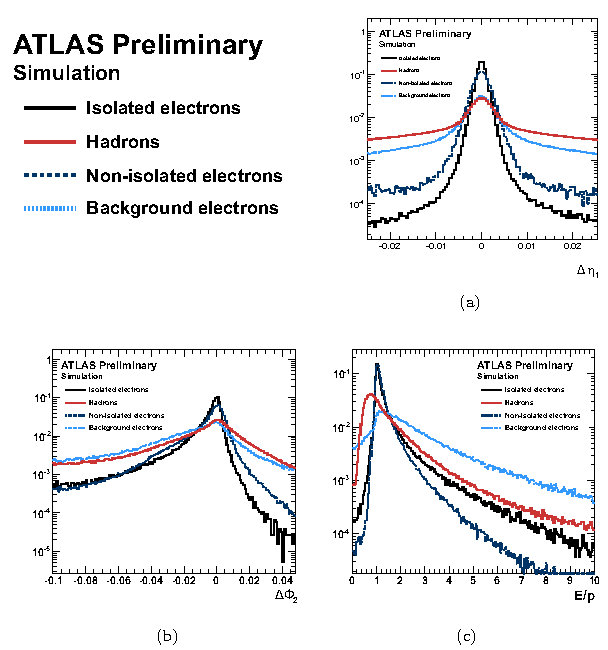
\includegraphics[width=12cm]{./textuais/identificacao/figuras/fig_3_variaveis_eletron.pdf}\\
	\caption{Variáveis combinadas de traço-calorimetria, mostrando a separação de vários tipos de background. As variáveis mostradas são: (a) diferença entre o traço e o \emph{cluster} de energia em $\eta$, (b) diferença entre o traço e o \emph{cluster} de energia em $\phi$, e (c) razão da energia medida no calorimetro com o momento medido no traço. Extraído de \cite{alison2014road}.}
	\label{fig:3T03}
\end{figure}

\begin{itemize}
  \item Variável de diferença entre o traço e o \emph{cluster} de energia em $\eta$, $\Delta$$\eta_1$:

  A comparação é feita extrapolando o traço até o calorímetro EM e esta distribuição é mais reduzida para os elétrons reais, portanto, a exigência de valores pequenos de $\Delta$$\eta$ reduz o ruído de fundo.

  \item Variável de diferença entre o traço e o \emph{cluster} de energia em $\phi$, $\Delta$$\phi_2$:

  Semelhante a variável descrita anterior, entretanto, menos discriminante devido aos fótons da radiação de Bremsstrahlung causarem uma diferença entre a posição do traço e o cluster em $\phi$.

  \item Variável de diferença entre o traço e o \emph{cluster} de energia em $\phi$, reescalada, $\Delta$$\phi_{res}$:

  É a variável $\Delta$$\phi_2$, porém com o momento de traço reescalado para a energia do \emph{cluster} depois da extrapolação para a camada central.

  \item Variável de razão entre a energia medida no calorímetro pelo momento determinado no ID, E/P:

  Como os hádrons não depositarão toda sua energia no EM, uma fração será depositada no HAD. A exigência de que E/P seja consistente com a expectativa de um elétron real pode suprimir tanto hádrons e quanto conversões.

\end{itemize}

\subsection{Variáveis de Isolamento}

Por último, as variáveis de isolamento também são utilizadas para discriminar sinal e ruído de fundo, são elas:

\begin{itemize}
  \item Et$_{cone}$;
  \item Pt$_{cone}$.
\end{itemize}

O isolamento é medido pela quantidade de energia próxima do elétron reconstruído, uma vez que elétrons de ruído de fundo são produzidos juntamente com outras partículas, o que os leva a ter maiores valores nessas variáveis. Dessa forma, essas variáveis conseguem ajudar na identificação de sinal e ruído de fundo

\section{Algoritmos Offline de Referência para a Identificação de Elétrons}

A colaboração ATLAS utiliza alguns algoritmos \emph{offline} para identificação de elétrons. Nessa seção, serão apresentados dois algoritmos, o e/$\gamma$, que é o padrão da colaboração e o algoritmo baseado em Verossimilhança, (do inglês, \emph{Likelihood}), que é a metodologia utilizada nessa dissertação.

\subsection{ATLAS e/$\gamma$}

O algoritmo e/$\gamma$ de seleção e identificação de elétrons, tem como princípio o corte baseado nas variáveis discriminantes. A utilização deste método como padrão traz a vantagem de compartilhamento e cruzamento de análises entre as diversas linhas de pesquisa no ATLAS \cite{aad2012performance}.

Como o intuito desta ferramenta é de ser compatível com o maior número possível de pesquisas físicas, três pontos de operação são disponibilizados \cite{alison2014road}:

\begin{description}
\item[\emph{Loose}] Nível de detecção de sinal elevado; entretanto, com a pior rejeição de ruído de fundo entre os três;
\item[\emph{Tight}] Melhor rejeição de ruído de fundo, por conseguinte, menor nível de eficiência entre os três.
\item[\emph{Medium}] Apresenta o ponto de equilíbrio entre os dois primeiros, com nível de rejeição de ruído melhor que o \emph{Loose} e eficiência melhor do que o \emph{Tight}.
\end{description}

Esses pontos de operação são configurados de forma que o \emph{Loose} seja um subconjunto de \emph{Medium} que é um subconjunto do \emph{Tight}, como mostra a Tabela~\ref{tab:01}; entretanto, com valores de cortes um pouco diferentes.

\begin{table}
  \centering
  \caption{Sumário das variáveis usadas nos critérios \emph{Loose++}, \emph{Medium++} e \emph{Tight++} do isEM++. Extraído de \cite{alison2014road} }\label{tab:01}
\begin{tabular}{c}

\textbf{Loose++}	\\ 	\hline
Shower shapes: R${_\eta}$, R${_{had1}}$ (R${_{had}}$, w${_2}$, E${_{ratio}}$,  w${_{s,tot}}$	\\ 	
Track quality	\\ 	
|${\Delta\eta}$| < 0.015	\\ 	
	\\ 	
\textbf{Medium++}	\\ 	\hline
Shower shapes: Same variables as Loose++, but at tighter values	\\ 	
Track quality	\\ 	
|${\Delta\eta}$| < 0.005	\\ 	
N${_{BL}}$ $\ge$ 1 for ${\eta}$ < 2.01	\\ 	
N${_{Pix}}$ > 1 for ${\eta}$ > 2.01	\\ 	
Loose TRT HT fraction cuts	\\ 	
|d0| < 5 mm	\\ 	
	\\ 	
\textbf{Tight++}	\\ 	\hline
Shower shapes: Same variables as Medium++, but at tighter values	\\ 	
Track quality	\\ 	
|${\Delta\eta}$|  < 0.005	\\ 	
N${_{BL}}$ $\ge$ 1 for all ${\eta}$	\\ 	
N${_{Pix}}$ > 1 for ${\eta}$ > 2.01	\\ 	
Tighter TRT HT fraction cuts	\\ 	
|d0| < 1 mm	\\ 	
E/P requirement	\\ 	
|${\Delta\phi}$|   requirement	\\ 	
Conversion bit	\\ 	

	
  %\hline
\end{tabular}
\end{table}
	
O perfil dos pontos de operação do e/$\gamma$, em 2011,  ganhou uma versão mais atualizada, e seus pontos de operação são chamados: \emph{Loose++}, \emph{Medium++} e \emph{Tight++}.


\subsection{Verossimilhança} \label{sec:likelihood}

Dentre as técnicas multivariadas existentes, a verossimilhança apresenta a vantagem de uma construção simples, no caso de independência entre as variáveis.

O método de verossimilhança faz uso de \ac{PDF} das variáveis discriminantes de sinais e de ruído de fundo para encontrar a probabilidade total. No algoritmo de verossimilhança do ATLAS, as PDF foram feitas por uma ferramenta da colaboração chamada \emph{\ac{TMVA} adaptative KDE}, que utiliza um método não-paramétrico chamado \ac{KDE} \cite{therhaag2012tmva}.


\subsubsection{O método da Verossimilhança}

O método de verossimilhança é uma função dos parâmetros de um modelo estatístico que permite inferir sobre o seu valor a partir de um conjunto de observações. No caso de identificação de elétrons do ATLAS, esse conjunto de observações são as variáveis discriminantes. Primeiramente, são construídas as PDF a partir dos dados de sinal e ruído de fundo. Com a consideração de independência entre as variáveis, as probabilidades conjuntas de sinal e ruído de fundo podem ser calculadas através de uma simplificação do método de verossimilhança, como mostram as equações~\ref{eq:04} e \ref{eq:05} \cite{atlas2014electron}.

\begin{equation}\label{eq:04}
    {L_s}\left( x \right) = \prod\limits_{a = 1}^m {{P_{s,a}}({x_a})}
\end{equation}

\begin{equation}\label{eq:05}
    {L_b}\left( x \right) = \prod\limits_{a = 1}^m {{P_{b,a}}({x_a})}
\end{equation}
onde ${{P_{s,a}}({x_a})}$ e ${{P_{b,a}}({x_a})}$ são as probabilidades associadas a cada uma das $m$ variáveis ($x_i$) do evento analisado. L$_{s}$ e L$_{b}$ são os valores da multiplicação da verossimilhança para sinal e ruído de fundo.

Com as duas probabilidades conjuntas calculadas, faz-se o discriminante, utilizando a equação \ref{eq:06}, onde dL é o discriminante.

\begin{equation}\label{eq:06}
    dL = \frac{{Ls}}{{Ls + Lb}}
\end{equation}

Construir o menu para a verossimilhança consiste em: escolher as variáveis, selecionar cortes adicionais e definir o valor de limiar do discriminante \cite{atlasdescription}, sendo que a eficiência da verossimilhança será o resultado da eficiência do discriminante e os cortes adicionais combinados.

Uma das principais diferenças entre o algoritmo e/$\gamma$ e a verossimilhança está nos eventos de cauda da PDF, uma vez que o primeiro efetua cortes rígidos, impossibilitando assim a classificação destes \cite{atlasdescription}.

\subsubsection{Verossimilhança para Elétrons no ATLAS}
	

O método de verossimilhança para identificação de elétrons apresenta cinco pontos de operação: \emph{Very Tight, Tight, Medium, Loose, Very Loose}, cada um com diferentes níveis de rejeição de ruído e eficiência de sinal, e estes pontos diferem entre si pelas variáveis e limiar dos cortes adicionais, como mostra a Tabela~\ref{tab:06}.

\begin{table}[h!]
  \centering
  \caption{Variáveis usadas na construção da verossimilhança para diferentes pontos de operação. Extraído de \cite{atlasdescription}.}\label{tab:06}
\begin{tabular}{c|c|c|c}

Menu	&	VERY TIGHT, TIGHT	&	MEDIUM	&	LOOSE, (VERY LOOSE)	\\ 	\hline
Variáveis da	&	R${_{Had}}$	&	R${_{Had}}$	&	R${_{Had}}$	\\ 	
Verossimilhança	&	R${_{\eta}}$	&	R${_{\eta}}$	&	R${_{\eta}}$	\\ 	
	&	F${_{HT}}$	&	F${_{HT}}$	&	F${_{HT}}$	\\ 	
	&	${\Delta\eta_{1}}$	&	${\Delta\eta_{1}}$	&	${\Delta\eta_{1}}$	\\ 	
	&	W${_{\eta2}}$	&	W${_{\eta2}}$	&	W${_{\eta2}}$	\\ 	
	&	f${_{1}}$	&	f${_{1}}$	&	f${_{1}}$	\\ 	
	&	f${_{3}}$	&	f${_{3}}$	&	f${_{3}}$	\\ 	
	&	E${_{ratio}}$	&	E${_{ratio}}$	&	E${_{ratio}}$	\\ 	
	&	R${_{\phi}}$	&	R${_{\phi}}$	&	R${_{\phi}}$	\\ 	
	&	$\Delta p/p$	&	$\Delta p/p$	&	$\Delta p/p$	\\ 	
	&	${\Delta\phi_{Res}}$	&	${\Delta\phi_{Res}}$	&	${\Delta\phi_{Res}}$	\\ 	
	&	d${_{0}}$	&	d${_{0}}$	&		\\ 	
	&	${\sigma _{{d_0}}}$	&	${\sigma _{{d_0}}}$	&		\\ 	\hline
Cortes	&	nSiHits $\ge$  7	&	nSiHits $\ge$  7	&	nSiHits $\ge$  7	\\ 	
Adicionais	&	nPixHits $\ge$ 2	&	nPixHits $\ge$ 2	&	nPixHits $\ge$ 2 ($\ge$ 1)	\\ 	
	&	Blayer	&	Blayer	&	Blayer (no Blayer)	\\ 	
	&	!(isConv)	&		&		\\ 	\hline
Comparar com	&	isTightPlusPlus	&	MediumPlusPlus	&	isLoosePlusPlus	\\ 	
	&		&		&	Multilepton	\\ 	

\end{tabular}
\end{table}
